%!TeX root = ../main.tex
\chapter{电子回旋辐射数值诊断}
\section*{引言}
%电子回旋辐射在等离子体中伴随着吸收和发射过程。等离子体若发射某一频率的辐射,也必将吸收同一频率的辐射。对于有辐射和吸收的等离子体,根据能量守恒条件,辐射输运方程可表示为
电子回旋辐射在输运中伴随着吸收和发射过程。介质若发射某一频率的辐
射,也必将吸收同一频率的辐射,因此介质对辐射输运过程起到重要作用。根据
基尔霍夫定律,辐射输运方程为
\begin{equation}
\mathrm{N}^{2} \frac{d}{d s}\left(\frac{\mathrm{I}}{\mathrm{N}^{2}}\right)=\eta_{\omega}-\alpha_{\omega} I
\end{equation}
其中$η_\omega$表示体辐射率,它表示单位体积等离子体沿入射辐射方向单位立体角的辐射功率,$α_\omega$表示体辐射吸收系数,N表示等离子体的折射率。在稀薄等离子体近似条件下,$N≈1$,这时辐射方程为
\begin{equation}\label{eq:dids}
\frac{d I}{d s}=\eta_{w}-\alpha_{w} I
\end{equation}
可见最终电子回旋辐射信号强度取决于路径s,等离子体辐射率$η_\omega$以及吸收系数$α_\omega$等。\par
本章主要目的是解决稀薄等离子体电子回旋辐射的计算问题,从单电子回旋辐射出发,计算等离子体辐射率$η_\omega$。接着着力解决辐射输运问题,包括射线追迹s、辐射吸收系数$α_\omega$等,最终建立完整的信号流程,为非热化电子动理学演化过程中电子回旋辐射提供数值诊断计算平台。
\section{等离子体辐射率}
在稀薄等离子体中$ω_{pe}/ω_{ce} ≪1$,等离子体自身的折射率接近于真空折射率,此时可以忽略折射率和电子-电子运动耦合对辐射的影响,等离子体电子回旋辐射可以通过单电子回旋辐射统计求和的方式给出\cite{RN1898}。本章所有计算都是在这一默认前提下完成。
\subsection{单电子回旋辐射}
如\autoref{fig:elecorb}所示,均匀磁场背景中,单电子绕磁力线螺旋运动产生的单位时间单位频率单位立体角的辐射谱可以表示为(见附录\autoref{sec:A1}):
\begin{equation}\label{eq:nw}
\eta_{1}(\omega, v, \theta)=\frac{e^{2} \omega^{2}}{8 \pi^{2} \varepsilon_{0} c} \sum_{1}^{\infty}\left|\begin{array}{c}-\hat{\mathrm{x}} \frac{\cos \theta}{\sin \theta}\left(\cos \theta-\beta_{\|}\right) J_{m}(\xi) \\-\hat{y} j \beta_{\perp} \frac{d J_{m}(\xi)}{d \xi} \\\hat{\mathrm{z}}\left(\cos \theta-\beta_{\|}\right) J_{m}(\xi)\end{array}\right|^{2} \delta\left[\left(1-\beta_{\|} \cos \theta\right) \omega-m \omega_{c e}\right]
\end{equation}
取模算符中向量$\hat{x}$、$\hat{y}$、$\hat{z}$表示辐射电磁波的偏振方向,$θ$表示观测方向和磁场方向的夹角。当$θ=π/2$时,电磁波的传播模式可分为X波和O波,其中X波电场振动方向垂直于磁场和传播方向($\hat{y}$方向),O波电场振动方向平行于磁场方向($\hat{z}$ 方向)。$\hat{q}$为传播方向,平行于$\hat{q}$方向的电场具有纵波特征。当$θ≠π/2$时,具有类似O、X波极化方向的电磁波对应功率分别表示为:
\begin{subequations}\label{eq:etapp}
\begin{align}
\eta_{1}^{\|}(\omega, \beta, \theta)&=\frac{e^{2} \omega^{2}}{8 \pi^{2} \varepsilon_{0} c}\sum_{1}^{\infty}\left|\hat{\mathrm{z}}\left(\cos \theta-\beta_{\|}\right) J_{m}(\xi)\right|^{2} \delta\left[\left(1-\beta_{\|} \cos \theta\right) \omega-m \omega_{c e}\right]\\
\eta_{1}^{\perp}(\omega, \beta, \theta)&=\frac{e^{2} \omega^{2}}{8 \pi^{2} \varepsilon_{0} c}\sum_{1}^{\infty}\left|-\hat{y} j \beta_{\perp} \frac{d J_{m}(\xi)}{d \xi}\right|^{2} \delta\left[\left(1-\beta_{\|} \cos \theta\right) \omega-m \omega_{c e}\right]
\end{align}
\end{subequations}

其中$∥(⊥)$表示电场平行(垂直)于磁场的电磁波。考虑所有偏振方向,总辐射功率为:
\begin{equation}
\eta_{1}(\omega, v, \theta)=\frac{e^{2} \omega^{2}}{8 \pi^{2} \epsilon_{0} c}  \sum_{1}^{\infty}\left[\begin{array}{c}\left(\frac{\cos \theta-\beta_{\|}}{\sin \theta}\right)^{2} J_{m}^{2}(\xi) \\+\beta_{\perp}^{2} J_{m}^{\prime2}(\xi)\end{array}\right] \delta\left[\left(1-\beta_{\|} \cos \theta\right) \omega-m \omega_{c e}\right]
\end{equation}
其中$J_m$表示第一类m阶贝塞尔函数,$ξ=(ωβ_⊥)/ω_{ce} sinθ$,$ω_{ce}=\frac{eB_0}{γm_e} $。
\begin{figure}[ht]
\centering
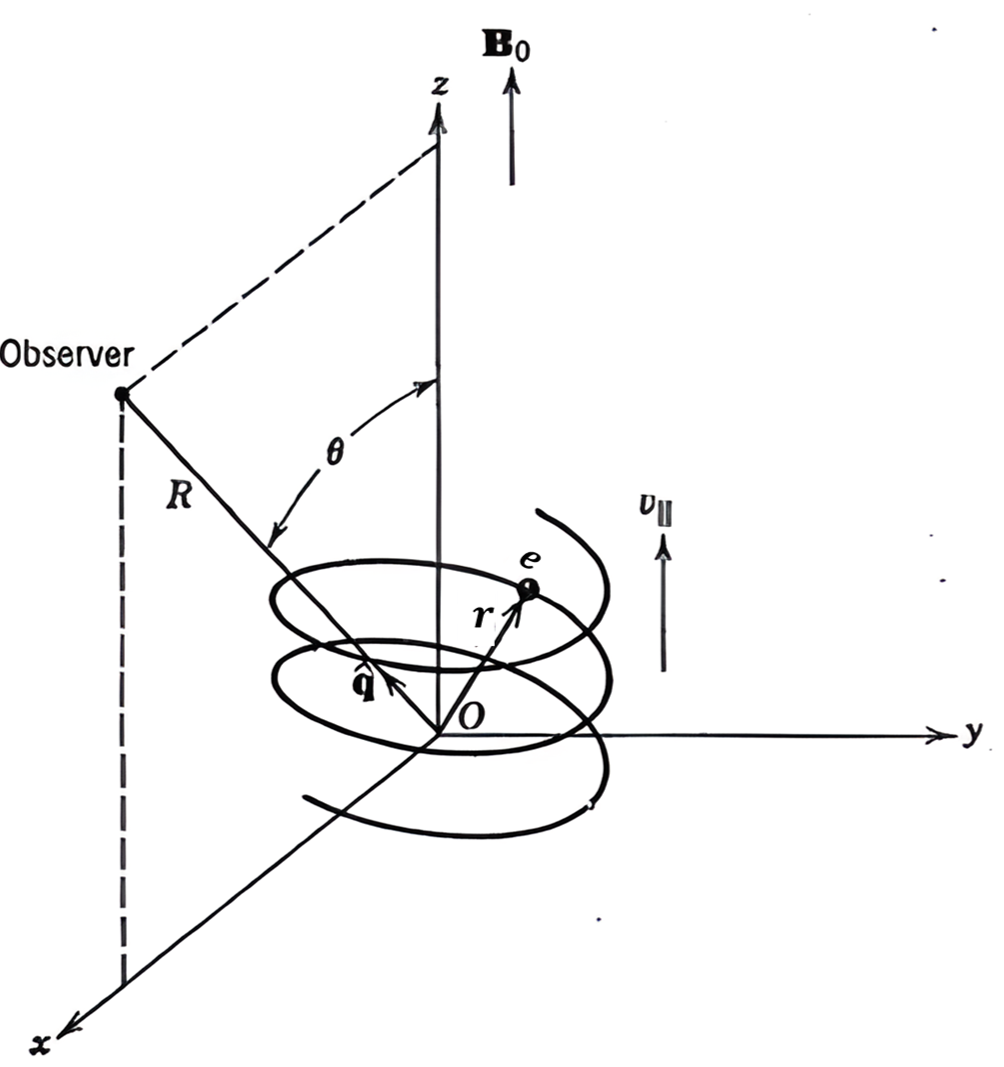
\includegraphics[width=12cm]{image50.png}
\caption{\label{fig:elecorb}均匀磁场中电子螺旋运动图}
\end{figure}
由\autoref{eq:nw}可知电子回旋辐射谱是由m=1、2、3…..一系列δ函数分立谱组成,即理论上电子回旋辐射是有无穷个谐频谱组成,对应的谐频频率为: 
\begin{equation}\label{eq:resonant}
\omega=\frac{m \omega_{\mathrm{ce}}}{1-\beta_{\|} \cos \theta}=\frac{{m \omega_{\mathrm{c} 0}}/{\gamma}}{1-\beta_{\|} \cos \theta}
\end{equation}
其中分母$(1-β_∥ cosθ)$和多普勒频移有关,$γ$和相对论频移有关。由于电子具有一定的速度分布,因此对于任一固定的 m 
次谐频,它都会有一定的频率展宽,称之为共振层,在该共振层内辐射频率、电子速度满足
\begin{equation}
\left(1-\beta_{\|} \cos \theta\right) \omega-m \omega_{c e}=0
\end{equation}
对于ECEI,理论上接收方向垂直于纵向磁场,取$θ=π/2$,这时候共振层主要依赖于相对论效应。考虑电子回旋基频为45GHz,对于85Ghz的辐射信号,其2、3、4次谐频共振曲线如\autoref{fig:resonant}所示,不同谐波共振层都是标准圆,谐波次数越高,圆半径越大,满足共振层条件的电子所需能量越高。但是限于空间条件或实验要求,接收方向和磁场方向夹角并不一定是严格90度,为了更加直观,这里取夹角$θ=π/3$,得到如\autoref{fig:resonant}所示的虚线,由于多普勒效应出现,共振曲线变成了椭圆。共振意味着波和粒子可以发生强烈的相互作用,比如外部入射的电磁波可以把能量传递给相应的粒子,因此根据椭圆共振层特征还可以实现等离子体平行方向电子速度分布测量。例如对于$f_{ce}/f\sim1$的微波信号以$cosθ=0.4(N_∥=0.4)$角度穿过处在匀强磁场中的等离子体,如\autoref{fig:resonant2}所示,当电子能量E<200keV时,垂直磁场方向温度$T_e<10keV$,对于不同的频率可认为只有唯一的$p_∥$与之发生共振。此时吸收系数完全由平行方向速度分布函数确定,通过测量不同频率信号的透射率就可以实现平行方向速度分布诊断\cite{RN1413}。
\begin{figure}[ht]
\centering
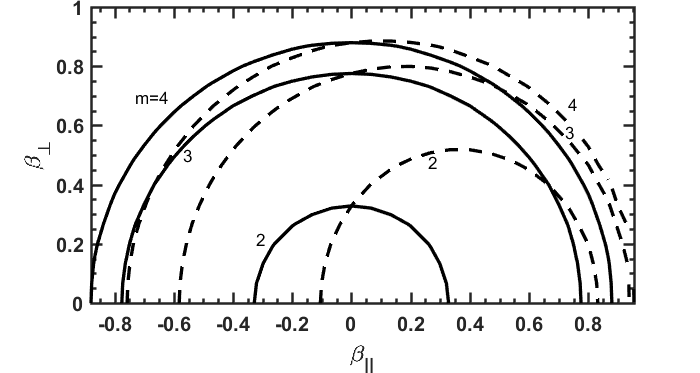
\includegraphics[width=12cm]{image51.png}
\caption{\label{fig:resonant}基频$ω_{c0}=45GHz$,辐射频率$ω=85GHz$,传播方向垂直于磁场(实线)和与磁场夹角$θ=π/3$(虚线)时不同谐波的共振层形状}
\end{figure}
\begin{figure}[ht]
\centering
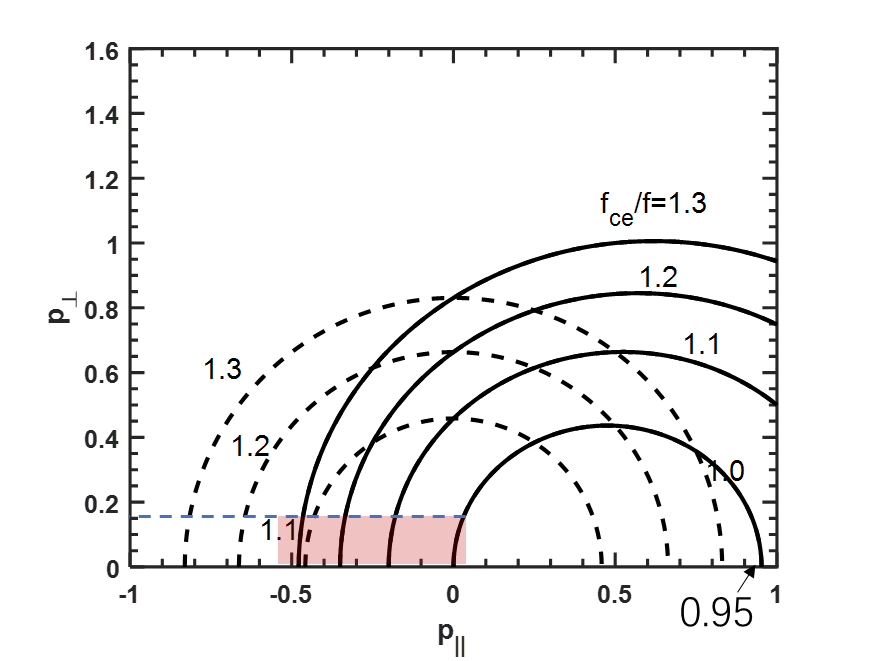
\includegraphics[width=12cm]{image52.png}
\caption{\label{fig:resonant2}不同频率下 $N_∥=0$(黑色虚线)和$N_∥=0.4$(黑色实线)共振曲线,其中$p_⊥ $、$p_∥ $表示约化动量,约化因子为$m_e c$ ,蓝色虚线对应垂直方向温度为10$keV$时所对应的平均垂直动量}
\end{figure}
\subsection{磁化等离子体电子回旋辐射}
当等离子体足够稀薄,自由空间处理是适用的,同时假设各个电子的辐射是不相关的,我们只需要对所有单个电子辐射强度简单求和从而获得等离子体的发射率。考虑归一化分布函数为$f(β_∥,β_⊥ )$,密度为$n_0$的等离子体,等离子体辐射率则表示为
\begin{equation}\label{eq:etawint}
\eta_{\omega}=n_{0} c^{3} \iint \eta_{1}  2 \pi \beta_{\perp} f\left(\beta_{\|}, \beta_{\perp}\right) d \beta_{\perp} d \beta_{\|}
\end{equation}
由\autoref{eq:etapp}和\autoref{eq:etawint}得:
\begin{equation}
\begin{aligned}\eta_{\mathrm{w}}^{\perp, \|}=n_{0} c^{3} & \sum_{m=1}^{+\infty} \iint d \beta_{\perp} d \beta_{\|}  \\& \times Q^{\perp, \|} \delta\left[\left(1-\beta_{\|} \cos \theta\right) \omega-m \omega_{c e}\right] \cdot 2 \pi \beta_{\perp} f\left(\beta_{\|}, \beta_{\perp}\right)\end{aligned}
\end{equation}
其中$Q^{(⊥,∥)}$分别为
\begin{subequations}
\begin{align}
Q^{\perp} & = \frac{e^{2} \omega^{2}}{8 \pi^{2} \epsilon_{0} c}\left[\beta_{\perp}^{2} J_{m}^{\prime 2}(\xi)\right] \\
Q^{\|} & = \frac{e^{2} \omega^{2}}{8 \pi^{2} \epsilon_{0} c}\left[\hat{\mathrm{z}}\left(\cos \theta-\beta_{\|}\right) J_{m}(\xi)\right]^{2}
\end{align}
\end{subequations}
这里$Q^⊥$ 、$Q^∥$分别表示电场方向垂直和平行于背景磁场的电磁波辐射算符(即X波和O波) 。辐射展宽的机制主要有两类,分别为相对论展宽$(1-β^2 )^{1/2}$和多普勒展宽$(1-β_∥ cosθ)^{-1}$。除此之外还有由于辐射导致电子能量指数衰减的自然展宽以及碰撞导致的碰撞展宽,相对于前两种展宽,之后的两种展宽可以忽略不计\cite{RN1900}。求解积分主要困难来自于积分项中二维狄拉克函数,解决方式是把二维积分通过狄拉克函数的性质转化为一维积分,具体方法可参考附录\autoref{sec:A3}。\par
  这里为了展示热分别状态下辐射率的频谱分布,假设等离子体速度分布为各项同性且满足麦氏分布,不考虑相对效应,分布函数可表示为:
\begin{equation}
f\left(\beta_{\|}, \beta_{\perp}\right)=\left(\frac{m_{e}}{2 \pi T}\right)^{\left(\frac{3}{2}\right)} \exp \left[\frac{m_{e} c^{2}\left(\beta_{\perp}^{2}+\beta_{\|}^{2}\right)}{2 T}\right]
\end{equation}\par
考虑ECEI接收到的电磁波为X模,且垂直纵场方向,取$Q=Q^⊥$,$θ=π/2$,$T=5~keV$, $n_e=10^{19}~m^{-3}$,根据$η_\omega^⊥$计算可得辐射频谱如\autoref{fig:spece}所示,信号强度主要集中在基频和二次谐频上,且谐频分布彼此重叠较小,更高次谐频之间相互重叠区域较大,分辨度小,且强度较低。因此电子回旋辐射诊断主要选取基频和二次谐频,保证了信号强度号和谐频成分的单一性。同时为了保证信号能传出托卡马克,对于X模通常选择二次谐频,对于O模通常选取基频(可参考\autoref{sec:ECEI})。
\begin{figure}
\centering
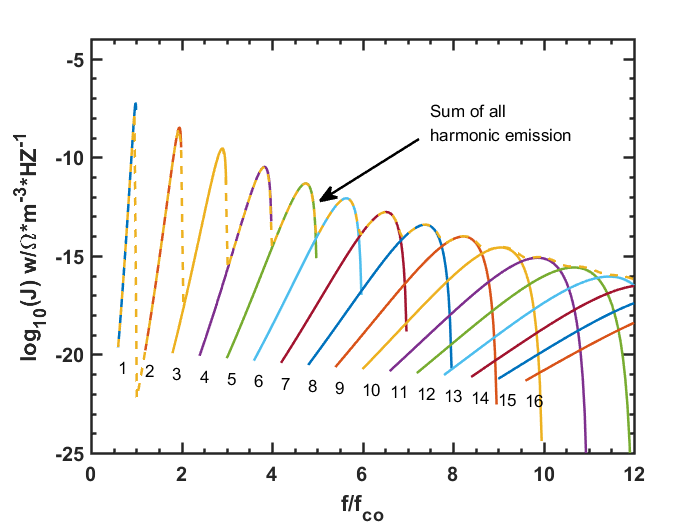
\includegraphics[width=14cm]{image53.png}
\caption{\label{fig:spece}温度为5keV,$f_{c0}=50GHz$,$n_e=10^{19}/m^3$时电子回旋辐射频谱图}

\end{figure}
\clearpage
\section{等离子体吸收系数}
\subsection{局部热平衡态下等离子体吸收系数}
当等离子体处于温度为$T_e$的局部热平衡态,单位路径吸收的电磁波能量和辐射的能量达到动态平衡。根据基尔霍夫定理,有
\begin{equation}
\eta_{\omega}-\alpha_{\omega} I_B=0
\end{equation}
吸收系数为
\begin{equation}\label{eq:alphaT}
\alpha_{\omega}=\frac{\eta_{\omega}}{I_B}
\end{equation}
普朗克黑体辐射表面亮度$I_B$(单位面积单位立体角辐射功率)可表示为
\begin{equation}
\mathrm{I}_{B}(\omega)=\frac{\hbar \omega^{3}}{4 \pi^{3} c^{2}} \frac{1}{e^{\frac{\hbar \omega}{T_{e}}}-1}
\end{equation}
考虑$ℏω≪T_e$,泰勒展开取一阶量得到
\begin{equation}\label{eq:Black}
\mathrm{I}_{B}(\omega)=\frac{T_{e} \omega^{2}}{4 \pi^{3} c^{2}}
\end{equation}
因此在满足黑体条件下辐射强度正比与温度,进一步考虑线偏振电磁波,如X模或O模,$I_B$则为
\begin{equation}
\mathrm{I}_{B}(\omega)=\frac{T_{e} \omega^{2}}{4 \pi^{3} c^{2}} * \frac{1}{2}=\frac{T_{e} \omega^{2}}{8 \pi^{3} c^{2}}
\end{equation}
最终,在热平衡条件下,根据\autoref{eq:alphaT}等离子体吸收系数为:
\begin{equation}\label{eq:alphaT2}
\alpha_{\omega}=\eta_{\omega} * \frac{8 \pi^{3} c^{2}}{T_{e} \omega^{2}}
\end{equation}

\subsection{非热平衡态下等离子体吸收系数}
在上一小节中主要考虑的是热平衡条件下(电子速度分布满足麦克斯韦分布)等离子体吸收系数的计算,吸收系数$α_ω$根据发射系数通过基尔霍夫定律求得:$α_ω=η_ω/I_B $。如果电子速度分布不满足热平衡条件时,吸收系数的计算需要通过更精细的能量平衡方程求得。\par
首先假设等离子体的折射率n$\sim$1,辐射能量输运方程表达式:
\begin{equation}
\frac{\partial \mathrm{I}_{\omega}^{\mathrm{i}}}{\partial \mathrm{s}}=\eta_{\omega}^{i}-\alpha_{\omega}^{i} I_{\omega}^{i}
\end{equation}
i表示极化类型,这里$η_\omega^i$和$α_\omega^i$分别为
\begin{align}\eta_{\omega}^{\mathrm{i}} & = \int \eta_{1}^{i}(\boldsymbol{p}) f(\boldsymbol{p}) d \boldsymbol{p} \\ \alpha_{\omega}^{\mathrm{i}} & = \int \alpha_{1}^{i}(\boldsymbol{p}) f(\boldsymbol{p}) d \boldsymbol{p}
\end{align}
这里$ η_1^i (p)$ 表示单电子自发辐射率,如磁化等离子体中的\autoref{eq:nw},$α_1^i (p)$表示运动状态为$\vp$的电子吸收系数。根据光子的量子性特征,动量为$\vp'$态的电子辐射出一个光子后变成$\vp$态,根据动量守恒和能量守恒关系 : 
\begin{align}
\boldsymbol{p}_{\|} & = \boldsymbol{p}_{\|}^{\prime}-\hbar \boldsymbol{k}_{\|}\\ \epsilon & = \epsilon^{\prime}-\hbar \omega
\end{align}
其中$∥$表示与磁场方向平行,电子通过在平行磁场方向失去(获得)动量而发射(吸收)光子。动量为$\vp'$电子的受激发射系数$\chi_1^{i*}({p} \prime)$和受激发射率$\eta_1^{i*}({p} \prime)$之间满足关系$\eta_1^{i*}({p} \prime)=\chi_1^{i*}({p} \prime)I_{\omega}$,$I_{\omega}$为背景辐射强度。根据爱因斯坦系数关系,受激发射系数$\chi_1^{i*} (\vp' )$和自发发射率$η_1^{i} (\vp' )$满足\cite{RN1002,RN2117}:
\begin{equation}
\eta_{1}^{i}\left(\boldsymbol{p}^{\prime}\right)=\chi_{1}^{i *}\left(\boldsymbol{p}^{\prime}\right) \frac{\hbar \omega^{3}}{8 \pi^{3} c^{2}}
\end{equation}
动量为$\vp$电子的受激吸收系数和动量为$\vp'$电子的受激发射系数之间的关系满足
\begin{equation}
\alpha_{1}^{i *}(\boldsymbol{p})=\frac{\Omega_{{p} \prime}}{\Omega_{{p}}} \chi_{1}^{i *}\left(\boldsymbol{p}^{\prime}\right)
\end{equation}
$Ω_\vp$,$Ω_\vp'$分别表示动量$\vp$和$\vp'$状态的统计权重且$Ω_\vp'/Ω_\vp=\dif\vp'/\dif\vp$。
根据以上方程,辐射能量输运方程可表示为:
\begin{equation}
\begin{aligned}
\frac{\partial I_{\omega}}{\partial s} & =\int f\left(\boldsymbol{p}^{\prime}\right)\left[\eta_{1}^{i}\left(\boldsymbol{p}^{\prime}\right)+\eta_{1}^{*}\left(\boldsymbol{p}^{\prime}\right)\right] d \boldsymbol{p}^{\prime}-I_{w} \int f(\boldsymbol{p}) \alpha_{1}^{*}(\boldsymbol{p}) d \boldsymbol{p}  \\
& =\int f\left(\boldsymbol{p}^{\prime}\right) \eta_{1}^{i}\left(\boldsymbol{p}^{\prime}\right) d \boldsymbol{p}^{\prime}-I_{w} \frac{8 \pi^{3} c^{2}}{w^{2}} \int \eta_{1}^{i}\left(\boldsymbol{p}^{\prime}\right) \frac{\left[f(\boldsymbol{p})-f\left(\boldsymbol{p}^{\prime}\right)\right]}{\hbar w} d \boldsymbol{p}^{\prime} \\
& =\eta_{\omega}^{i}-I_{\omega} \alpha_{w}^{i} 
\end{aligned}
\end{equation}
其中
\begin{align}
\eta_{{\omega}}^{i} & = \int f\left(\boldsymbol{p}^{\prime}\right) \eta_{1}^{i}\left(\boldsymbol{p}^{\prime}\right) d \boldsymbol{p}^{\prime} \\
\alpha_{\omega}^{i} & = \frac{8 \pi^{3} c^{2}}{\omega^{2}} \int \eta_{1}^{i}\left(\boldsymbol{p}^{\prime}\right) \frac{\left[f(\boldsymbol{p})-f\left(\boldsymbol{p}^{\prime}\right)\right]}{\hbar \omega} d \boldsymbol{p}^{\prime}\label{eq:alpha1}
\end{align}
为了研究$α_\omega^i$,首先需要把$α_\omega^i$表示成数学可以处理的形式,不难发现
\begin{equation}\label{eq:fte}
f\left(\boldsymbol{p}^{\prime}\right)=f\left(\boldsymbol{p}_{\|}^{\prime}, \epsilon^{\prime}\right)=f\left(\boldsymbol{p}_{\|}+\frac{\hbar \omega}{c} \cos \theta, \epsilon+\hbar \omega\right)
\end{equation}
由于辐射出光子的动量远小于电子本身动量$(ℏk\ll \vp')$,辐射出的光子能量远小于电子本身携带的能量$(ℏω\ll ϵ')$,因此$f(\vp' )$可表示为一阶泰勒展开形式,
由\autoref{eq:alpha1}和\autoref{eq:fte}得:
\begin{equation}\label{eq:alpha2}
\alpha_{\omega}=-\frac{8 \pi^{3} c^{2}}{\omega^{2}} \int \eta_{1}^{i}\left(\boldsymbol{p}^{\prime}\right) \left[\frac{\partial f}{\partial p_{\|}} \cdot \frac{\cos \theta}{c}+\frac{\partial f}{\partial \epsilon}\right]\dif {\vp}^{\prime}
\end{equation}
根据文献记载,该方程最早由前苏联科学家TRUBNIKOV推导得到\cite{RN1344}。为了计算方便,本文中将积分坐标从$(p_∥,ϵ)$转化为$(p,ξ)$,其中p是约化因子为$m_ec$的约化动量,$\xi=p_{\|}/p$,最终形式为(可参考附录\autoref{sec:A2})
\begin{equation}
\alpha_{\omega}=-\frac{8n_{0} \pi^{3} c^{2}}{m_{e} c^{2} \omega^{2}} \int \eta_{1}^{i}(\beta, \xi)\left[\frac{1}{p} \frac{\partial f}{\partial \xi} \cos \theta+\frac{\sqrt{1+p^{2}}}{p} \frac{\partial f}{\partial p}-\frac{\xi \sqrt{1+p^{2}}}{p^{2}} \frac{\partial f}{\partial \xi}\right] 2 \pi p^{2}  \dif p \dif \xi
\end{equation}
当$ θ=π/2$,且分布函数满足麦克斯韦分布即$ f\sim \exp(-ϵ/T_e )$,由\autoref{eq:alpha2}得:
\begin{equation}
\alpha_{\omega}=\eta_{\omega} * \frac{8 \pi^{3} c^{2}}{T_{e} \omega^{2}}
\end{equation}
此时吸收系数退回到热平衡态的\autoref{eq:alphaT2}。\par
当等离子体满足热平衡条件时,光学厚度是决定辐射强度和温度关系的一个重要指标,根据等离子体输运方程\autoref{eq:dids},在不考虑壁反射条件下,最终接收到的信号强度满足方程:
\begin{equation}
I(s)=\frac{\eta_{\omega}}{\alpha_{\omega}}\left[1-e^{-\tau}\right]
\end{equation}
其中光学厚度的定义为
\begin{equation} \label{eq:tauN}
τ=∫α_\omega \dif s
\end{equation}
在满足局部热平衡条件时,根据\autoref{eq:alphaT2}
\begin{equation}
\frac{\eta_{\omega}}{\alpha_{\omega}}=I_{B}(T) \sim \frac{T_{e} \omega^{2}}{8 \pi^{3} c^{2}}
\end{equation}
因此只有当光学厚度$τ>1$时辐射强度才近似正比于温度$T_e$。
\subsection{两种光学厚度计算方法的对比}
本论文之后的吸收系数计算均采用上述利用爱因斯坦系数关系得到的\autoref{eq:alpha2}。我们将之与经典的局域热平衡等离子体光学厚度计算方法\cite{RN1952}进行进一步校验。以EAST托卡马克参数为环境背景,其大半径R0=1.85m,小半径a=0.45m。假设放电中纵场电流为IT=10000A,对应磁轴处磁场强度大约为2.25T。我们考虑两种密度分布环境,分别为低密度环境,对应磁轴中心密度为$n_{ea0}=7\times10^{18}m^{-3}$,以及高密度环境,对应磁轴中心密度为$n_{eb0}=3\times10^{19}m^{-3}$,芯部温度均为$T_{e0}=1keV$,进一步假设密度分布和温度分布满足二次分布:
\begin{align}
n_{e r} & =n_{e 0} \left(1-\rho^{2}\right)^{2} \label{eq:nr}\\
T_{e r} & =T_{e 0} \left(1-\rho^{2}\right)^{2}\label{eq:Tr}
\end{align}
其中$\rho$表示约化半径,$ρ<0$对应高场侧,$ρ>0$对应低场侧。我们通过计算不同半径处所对应的冷等离子体二次回旋频率光学厚度来对两种计算方法进行比较。\\
\noindent 1.通过爱因斯坦发射吸收系数计算光学厚度\par
利用Trubnikov\autoref{eq:alpha2}计算二次电子回旋频率在不同位置处吸收系数的分布,最后通过数值的方法计算吸收系数沿光学路径的积分,从而获得不同半径冷等离子体电子回旋频率对应的光学厚度。这里选择直线为积分路径,没有考虑等离子体的折射效应。\par
\noindent 2.从等离子体介电属性出发解析计算光学厚度\par
另一种求解吸收系数的方式是通过电磁波在等离子体中传播的能量输运方程,利用输运方程中单位路径的能量的吸收和能流之比来求解吸收系数,吸收系数可表示为\cite{RN1952}
\begin{equation}\label{eq:alphaBornatic}
\alpha=\left[(\omega / 4 \pi) \overrightarrow{\widetilde{E}}^{*} \cdot \overrightarrow{\varepsilon_{a}} \cdot \overrightarrow{\tilde{E}}\right] /|\vec{S}|
\end{equation}
其中
\begin{equation}
\vec{S}\left(\vec{k}^{\prime}, \omega\right) \equiv \frac{c}{4 \pi} \operatorname{Re}\left(\overrightarrow{\widetilde{E}} \times \vec{\widetilde{B}}^{*}\right)-\frac{\omega}{8 \pi} \frac{\partial \varepsilon_{h, i j}}{\partial \vec{k}^{\prime}} \widetilde{E}_{i}^{*} \tilde{E}_{j}
\end{equation}
$\overrightarrow{\widetilde{E}} $和$\vec{\widetilde{B}}$表示电磁波的电场和磁场,$\omega$为电磁波角频率,$\varepsilon_{h, i j}$和$\varepsilon_{a, i j}$分别为等离子体的实介电张量和虚介电张量,与分布函数的具体形式有关,$\vec{k}^{\prime}$为电磁波波矢。\autoref{eq:alphaBornatic}中分子表示等离子体对电磁波的吸收,分母表示能流。在满足局部热平衡条件下Bornatici根据\autoref{eq:alphaBornatic}推导出托卡马克中n次回旋频率$(n≥2)$光学厚度的计算公式如下\cite{RN351}:
\begin{equation}\label{eq:tauB}
\tau_{n}^{(X,O)}(\theta)=\frac{\pi n^{2(n-1)}}{2^{n}(n-1) !}\left(\frac{\omega_{p}}{\omega_{c}}\right)^{2}\left(\frac{T}{m_e c^{2}}\right)^{n-1}(\sin \theta)^{2(n-1)}\left(1+\cos ^{2} \theta\right) \mu_{n}^{(x, 0)}(\theta) \frac{\omega_{c} L_{B}}{c}
\end{equation}
其中$ω_p$表示等离子体频率,$ω_c$表示电子回旋频率、T表示等离子体温度,$L_B=\left(\frac{1}{B_{0}} \frac{\partial B_{0}}{\partial s}\right)^{-1}$表示纵场(纵向磁场)梯度标长,$θ$表示传播方向和背景磁场的夹角,$μ_n^{(X,O) }$定义为:
\begin{equation}
\mu_{n}^{(X, O)}(\theta) \equiv \frac{\left(N^{(x, 0)}\right)^{2 n-3}}{1+\cos ^{2} \theta} \frac{(n-1)^{2}\left[1-\left(n+\frac{1}{n}\right) f_{n}^{(X, O)}(\theta)\right]^{2}}{\left[\left(a_{n}^{2}+b_{n}^{2}\right)^{\frac{1}{2}}\right]_{N=N^{(X, O)}}}
\end{equation}
$a_n$和$b_n$的定义为:
\begin{align}
a_{n}^{2}& \equiv\left[1+\frac{\left[1-\left(\frac{\omega_{p}}{n \omega_{c}}\right)^{2}\right] N^{2} \cos ^{2} \theta}{\left[1-\left(\frac{\omega_{p}}{n \omega_{c}}\right)^{2}-N^{2} \sin ^{2} \theta\right]^{2}} n^{2}\left(1-\frac{n^{2}-1}{n^{2}} f_{n}^{(\mathrm{x}, \mathrm{o})}\right)^{2}\right]^{2} \sin ^{2} \theta \\
b_{n}^{2} &\equiv\left[1+\frac{1-\left(\frac{\omega_{p}}{n \omega_{c}}\right)^{2}}{1-\left(\frac{\omega_{p}}{n \omega_{c}}\right)^{2}-N^{2} \sin ^{2} \theta} n^{2}\left(1-\frac{n^{2}-1}{n^{2}} f_{n}^{(x, 0)}\right)^{2}\right]^{2} \cos ^{2} \theta
\end{align}
$N^2=\left [N^{(X,O)} \right]^2$和$f_n^{(X,O) }$的定义为:
\begin{align}
\left[N^{(X, O)}\right]^{2} = 1-\left(\frac{\omega_{p}}{n \omega_{c}}\right)^{2}& \frac{2\left[n^{2}-\left(\frac{\omega_{p}}{\omega_{c}}\right)^{2}\right]}{2\left[n^{2}-\left(\frac{\omega_{p}}{\omega_{c}}\right)^{2}\right]-\sin ^{2} \theta \mp  
\rho_{n}} \equiv 1-\left(\frac{\omega_{p}}{n \omega_{c}}\right)^{2} f_{n}^{(X, 0)}(\theta) \\
\rho_{n}^{2} \equiv \sin ^{4} &\theta+\frac{4}{n^{2}}\left[n^{2}-\left(\frac{\omega_{p}}{\omega_{c}}\right)^{2}\right]^{2} \cos ^{2} \theta
\end{align}
其中+表示X波,-表示O波。
\begin{figure}[H]
\centering
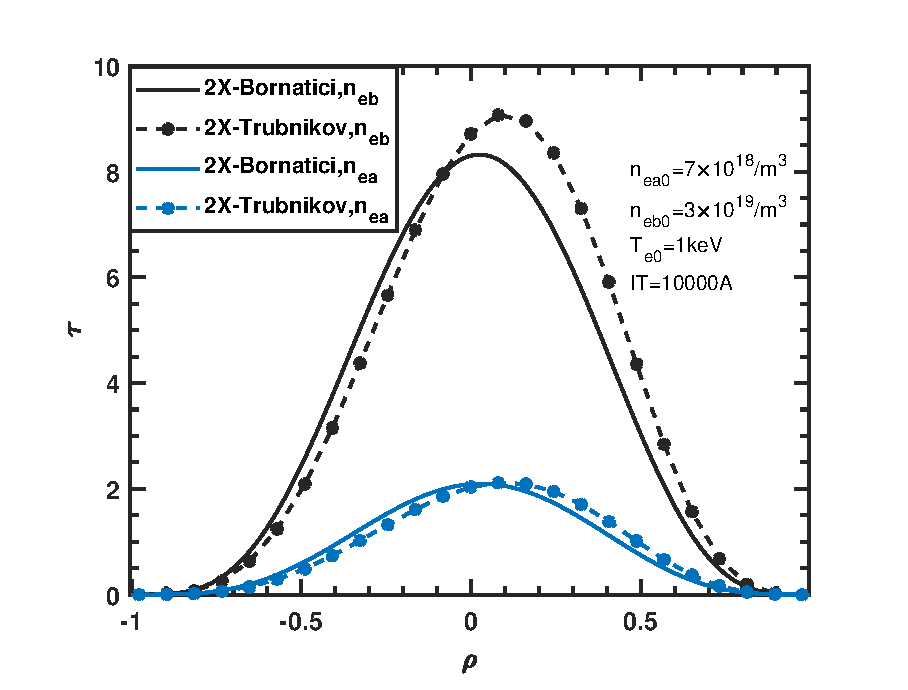
\includegraphics[width=14cm]{image55_2.eps}
\caption{\label{fig:tauc}两种光学厚度计算方法对比,黑色表示芯部密度为$3\times10^{19}/m^3$的高密度环境,蓝色表示芯部密度为$7\times10^{18}/m^3$的低密度环境}
\end{figure}
\par 两种方法得到的2X-mode光学厚度如\autoref{fig:tauc}所示,从图中可以看出两种方法在低密度环境下所得结果几乎完全一致。高密度环境下存在一定差别,原因是\autoref{eq:alpha2}多适用于稀薄等离子体,忽略了等离子体折射率对吸收系数的影响而解析方程\autoref{eq:tauB}在推导过程中也做了一定的近似。即使如此,在芯部密度为$3\times10^{19}/m^3$的高密度环境下,Trubnikov(\autoref{eq:alpha2})和Bornatici(\autoref{eq:tauB})所得结果相差也不超过13\%,因此可以断定Trubnikov方程在芯部密度为$(1-3)\times10^{19}/m^3$,磁场为$(2-3)T$等离子体环境中也应适用。但Trubnikov公式可以求解任意速度分布的等离子体吸收系数,Bornatici公式只能特定求解满足局部热分布的等离子体光学厚度,因此方程Trubnikov方程在解决非热化电子辐射中尤为重要。
\section{射线追迹}
前文介绍了稀薄等离子体辐射方程和吸收系数,在能量输运方程中,我们还需要考虑辐射路径问题。实验上我们是通过前端光路和天线来收集电子回旋辐射信号。那么每个电子的辐射的电磁波在空间中如何被我们的接收器收集?这里有一种直接求解的办法:把每个电子当作一个点源,利用接收器的边界条件,通过求解格林函数的办法去计算我们接收信号强度的大小。这样做显然是不容易的,因此2002年A .D .Piliya提出了另一种方法:利用光学互易原理逆向求解信号接收强度\cite{RN1367}。\par
互易关系常用在电路分析中,其性质是在只有一个电压源(或电流源),不含受控源的线性电阻电路中,电压源(或电流源)与电流表(电压表)互换位置,电流表读数不变,也就是说激励和响应互换位置之后,激励与响应的比值保持不变。如\autoref{fig:recp}所示,对于一个理想的互易电路(a)(b),电路传递函数$G21=G12$,其中$i_2=G21*u_s$,$i_1=G12*u_s$。因此对于一个未知的无源线性电阻电路系统,可以通过主动提供电流$i_1$测量$u_s$来获得$G12$,继而实现通过$u_s$监测$i_2$的变化。
\begin{figure}[ht]
\centering
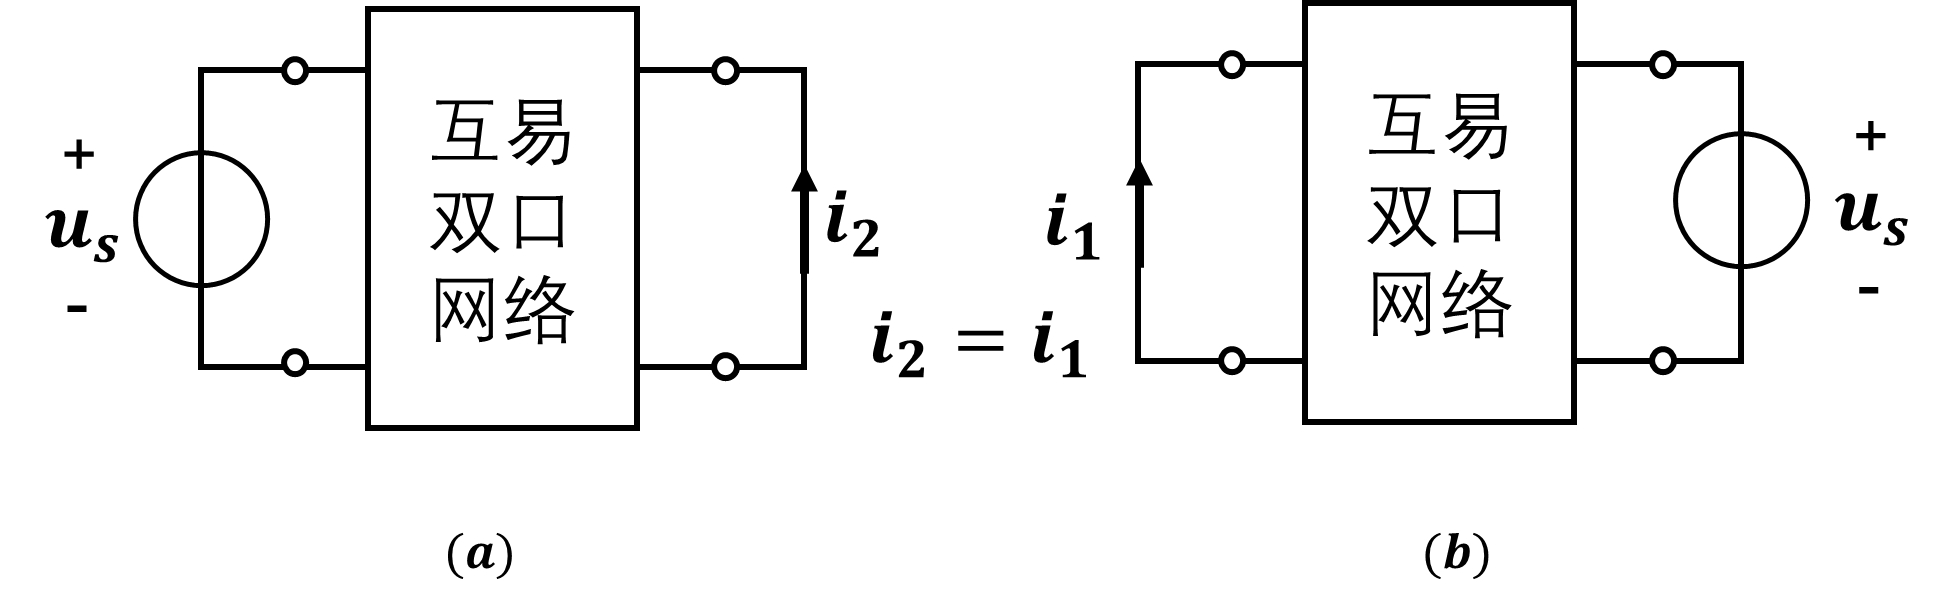
\includegraphics[width=14cm]{image55.png}
\caption{\label{fig:recp}电路互易原理}
\end{figure}
光学互易原理利用了物和像的对易关系,将等离子体中电子看成物,电子发射的电磁波经过ECEI光学系统后在接收器处的投影为像,系统所接收到的信号强度为光路中所有电子的像的叠加,因此只要找到物和像之间强度关系然后对整个光路中电子的辐射强度加权积分即可获得对应接收强度。物像之间的强度关系可以理解为系统对空间中不同位置电子辐射信号的收集效率。如\autoref{fig:recp_ece}所示,假设等离子体中电磁波的电场和磁场为$(\vE,\vH)$,天线接收到的电场波为$(\vE^{(out)},\vH^{(out)})$,光学收集效率为$A_{12}(\omega)$,则有
\begin{equation}
\left(\begin{matrix}
\vE^{(\text {out })} \\
\vH^{(\text {out })}
\end{matrix}\right)=A_{12}(\omega)\left(\begin{matrix}
\vE \\
\vH
\end{matrix}\right)
\end{equation}
同时,通过调换物像位置,将接收处视为发射处,发射频率等于接收频率,根据接收喇叭的边界条件,处在接收喇叭处激发的微波信号将会以高斯光束的结构发射出去,此时有
\begin{equation}
\left(\begin{matrix}
\vE^+ \\
\vH^+
\end{matrix}\right)=A_{21}(\omega)\left(\begin{matrix}
\vE^{(\text {in })} \\
\vH^{(\text {in })}
\end{matrix}\right)
\end{equation}
又因为光学系统满足对易原理,此时有$A_{12}=A_{21}$,而根据高斯光束的特征,$A_{21}$是容易求得的,这样就相当于获得光学系统中的$A_{12}$,该高斯光束所照亮的空间即表示接收光路的光学特征,高斯光束的强度分布则反应了不同位置处信号的收集效率,继而建立了当地电子回旋辐射强度$(E,H)$和接收信号强度$(E^{(out)},H^{(out)})$之间的关系。
\begin{figure}[H]
\centering
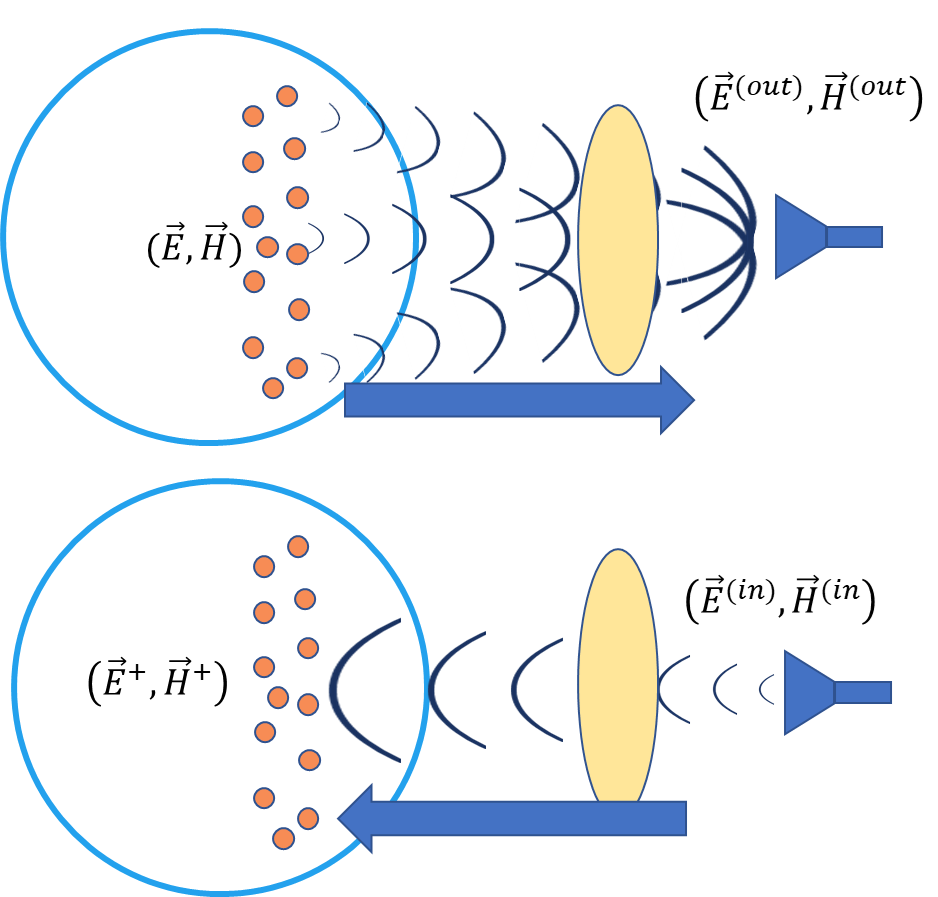
\includegraphics[width=10cm]{reciprocity.png}
\caption{\label{fig:recp_ece}电子回旋辐射诊断光路对易原理,上图表示实验中实际信号传播图,下图为调换物像的对易图,以接收器为发射器}
\end{figure}
在本文中,由于所有计算只是定性分析信号强度。为了减少计算复杂度,这里放弃了高斯光学空间积分,只考虑了几何光学路径积分。同时本文只考虑托卡马克中平面处沿径向方向的辐射信号,原则上只需要用直线路径计算即可,不需要考虑复杂的射线追迹,但开发3维射线追迹对研究电子回旋辐射信号也非常重要,因此本文将3维射线追迹程序开发思路也放在附录\autoref{sec:A4},以便参考。
\section{电子回旋辐射输运方程数值分析}
本章至此确定了电子回旋发射谱$η_\omega$计算、电子回旋吸收系数$α_\omega$计算、辐射路径s。在具备了计算回旋辐射的必要信息后,通过路径积分\autoref{eq:dids}即可得到接收到的回旋辐射强度,本节将从数值上模拟不同条件下最终接收到的回旋辐射强度I。
\subsection{局部热平衡条件下2X模电子回旋辐射}
这里以在中平面ECEI系统为研究对象,由于等离子体介电常数分布关于中平面近似上下对称,ECEI系统光路垂直于纵场方向,这时不需要考虑辐射路径偏折效应,辐射路径为直线。同样以EAST装置为研究背景,假设纵场电流$IT=10000A(B0=2.25T) $,中心电子密度$n_{e0}$为$1\times10^{19}m^{-3}$,电子温度$T_{e0}=2keV$,电子温度分布和密度分布满足\autoref{eq:nr}和\autoref{eq:Tr},如\autoref{fig:distri}(a)。以此背景探索不同频率的电子辐射随路径的变化关系以及辐射温度和当地电子温度之间的关系。
\begin{figure}[ht]
\centering
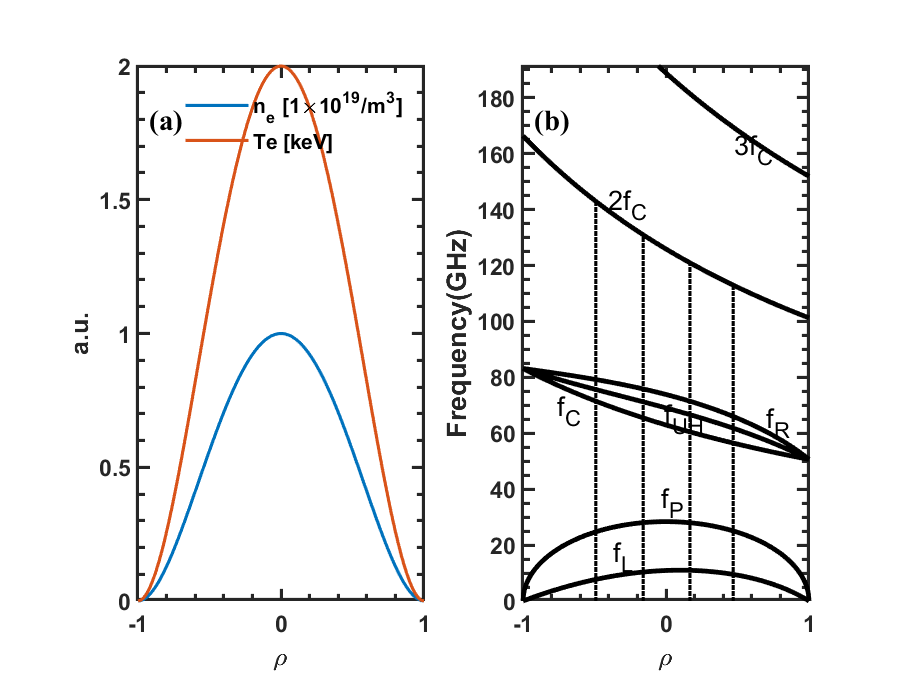
\includegraphics[width=14cm]{image56_1.eps}
\caption{\label{fig:distri}(a)电子密度分布以及温度分布.(b)特征频率分布,图中虚线分别表示频率为143Ghz、131Ghz、121Ghz以及113Ghz的2X波所对应的冷等离子体共振层位置}
\end{figure}
我们分别选取了频率为143Ghz、131Ghz、121Ghz以及113Ghz的2X波电子回旋辐射为研究对象,研究不同频率从高场侧传播到低场侧强度变化。各频率对应的冷等离子体共振层\footnote{注:冷等离子体共振层采用电子静止质量计算共振位置,未考虑相对论效应导致的质量变化,因此托卡马克中冷等离子体共振层位置是确定的}位置如\autoref{fig:distri}(b)中黑色虚线所示。
\par 求解各频率辐射强度大致分成三步:通过求解发射率\autoref{eq:etawint}以及吸收系数\autoref{eq:alpha2}式获得每一支频率发射率和吸收系数随半径的分布,结合辐射输运\autoref{eq:dids}式最终获得辐射强度随路径的分布。如\autoref{fig:Idistri}所示,(a)图为各频率发射率分布,(b)图为各频率吸收系数分布,(c)图表示各频率的辐射强度分布,其中黑色虚线对应不同频率的冷等离子体共振层位置,黑体辐射强度用绿线表示,用以比较黑体辐射强度和对应位置的电子回旋辐射强度。当黑体辐射强度和对应位置的电子回旋辐射强度相等时则意味着辐射温度和背景电子温度相等。从\autoref{fig:Idistri}中可以看出,在冷等离子体共振位置偏高场侧,相应的回旋辐射就已具有一定强度,这是由于相对论效应导致高场侧辐射频率下移,以至于共振层对应的冷等离子体电子回旋频率总是由高场侧等离子体贡献。
\begin{figure}[H]
\centering
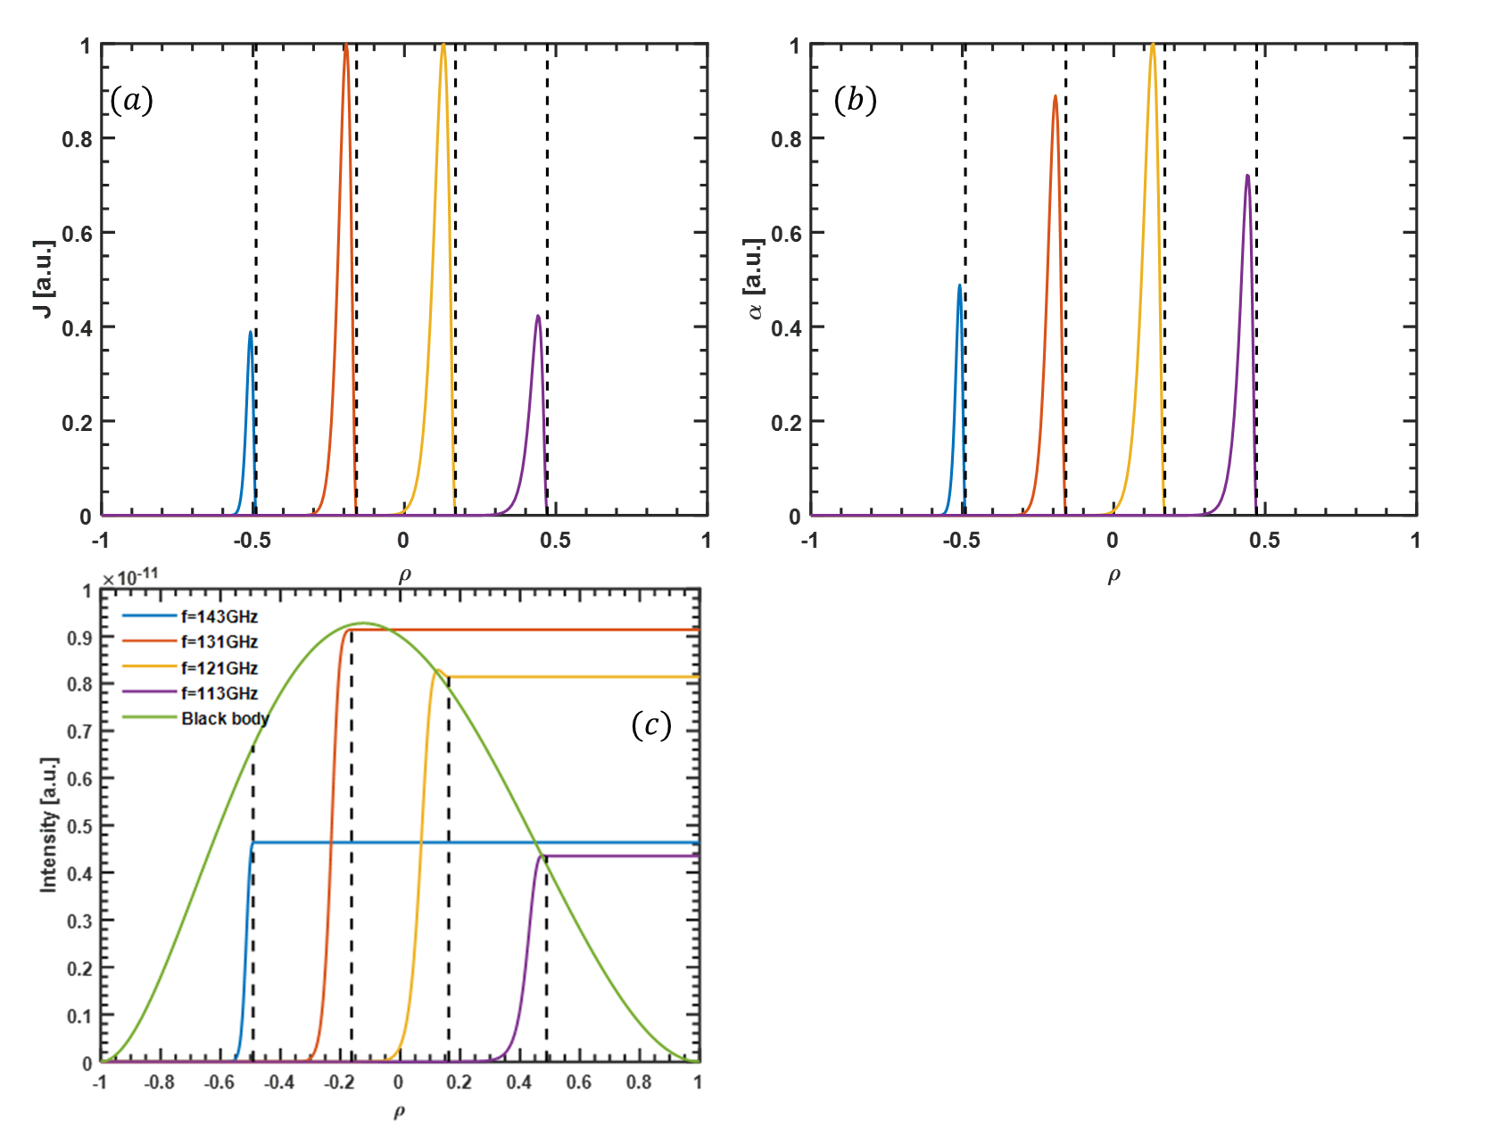
\includegraphics[width=12cm]{image57_1.png}
\caption{\label{fig:Idistri}不同频率发射率、吸收系数以及辐射强度随空间分布图。(a)发射率分布.(b)吸收系数分布.(c)辐射强度分布.图中绿线表示当地电子温度所对应的黑体辐射强度,黑色虚线表示各频率所对应的冷等离子体共振层位置。当辐射强度在其冷等离子体共振层处等于当地黑体辐射强度时,则辐射温度与当地电子温度相等.}
\end{figure}
%\begin{figure}[ht]
%\centering
%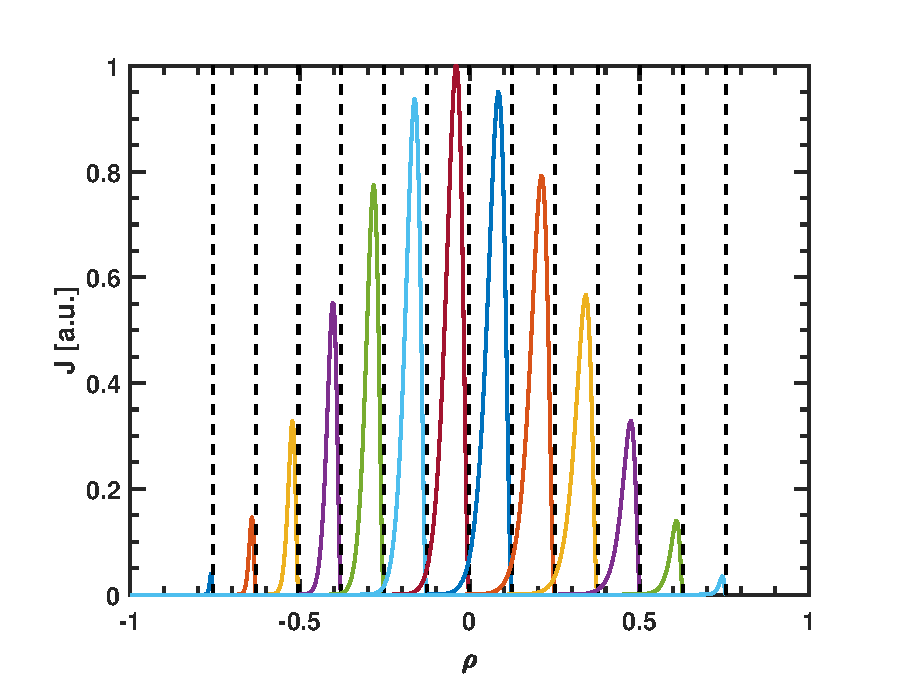
\includegraphics[width=12cm]{image58.eps}
%\caption{\label{fig:Adistri}不同频率的吸收系数分布,黑色虚线对应各频率的冷等离子体共振层位置}
%\end{figure}

为了检验利用电子回旋辐射测量电子温度的可靠性,这里进一步将径向位置从内到外分成24个测量点,收集每个测量点所对应的冷等离子体二次电子回旋频率辐射强度,利用\autoref{eq:Black}计算每个频率的辐射温度,进而获得辐射温度分布,如\autoref{fig:Taudistri}(b)所示。
同时我们还可以对吸收系数路径积分获得每个位置的光学厚度,如\autoref{fig:Taudistri}(a)所示。由于共振层厚度与纵场梯度标长$L_B$(\autoref{eq:tauB})呈正比,高场侧共振层厚度普遍小于低场侧,因此高场侧较低场侧更难达到光学厚条件。从光学厚度图中可以看出只有在约化半径$ρ\in(-0.4\sim0.6)$区间满足光学厚度远大于1的条件(这里的大于2就算远大于1了,因为它是关于自然数e的指数函数),因此也只有在$ρ∈(-0.4,0.6)$区间辐射温度才能近似等于电子温度。在边缘处由于光学厚度不满足远大于1条件,辐射温度偏离实际电子温度较大。如果我们仔细观测\autoref{fig:Taudistri}(b)则会发现,即使在满足光学厚度条件下,辐射温度也并不严格等于当地电子温度,而且这种不相等的特征表现为高场侧辐射温度低于背景电子温度,而低场侧辐射温度略高于背景电子温度。导致这种现象的部分原因是我们在计算过程中没有对位置作相对论修正,频率与位置对应关系仍采用冷等离子体处理。实际上由于相对论效应导致频率下移,每一个径向位置的冷等离子体共振频率事实上来源于更高场侧的电子贡献,低场侧每个位置的冷等离子体共振频率所对应的辐射实际上是由更靠近芯部的电子贡献,因此辐射温度略高于当地电子温度,而高场侧每个位置的冷等离子体共振频率所对应的辐射实际上是由更远离芯部的电子贡献,因此辐射温度略低于当地电子温度。随着托卡马克温度上升,这种效应也会更加明显,但是我们也可以通过反向偏移频率修正位置偏差。根据共振频率\autoref{eq:resonant}

\begin{figure}[H]
\centering
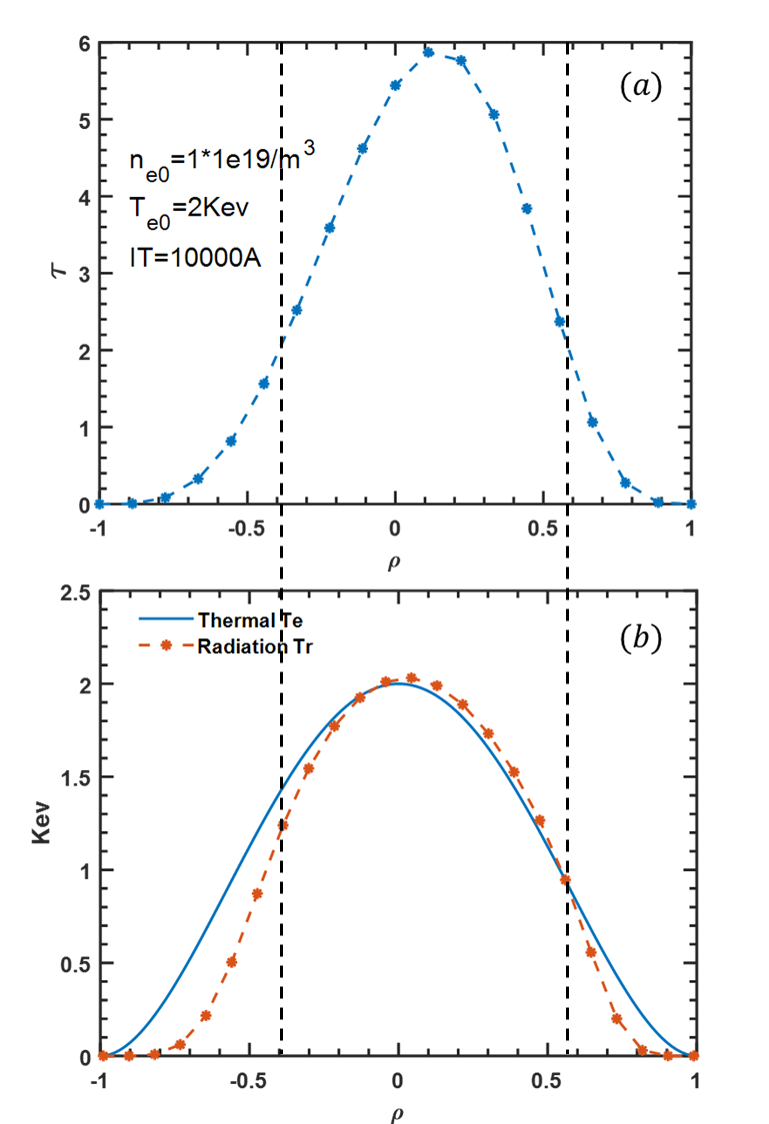
\includegraphics[width=12cm]{image59_1.png}
\caption{\label{fig:Taudistri} (a)光学厚度.(b)辐射温度与热温度.黑色虚线之间光学厚度大于2,满足光学厚条件}
\end{figure}

\begin{figure}[H]
\centering
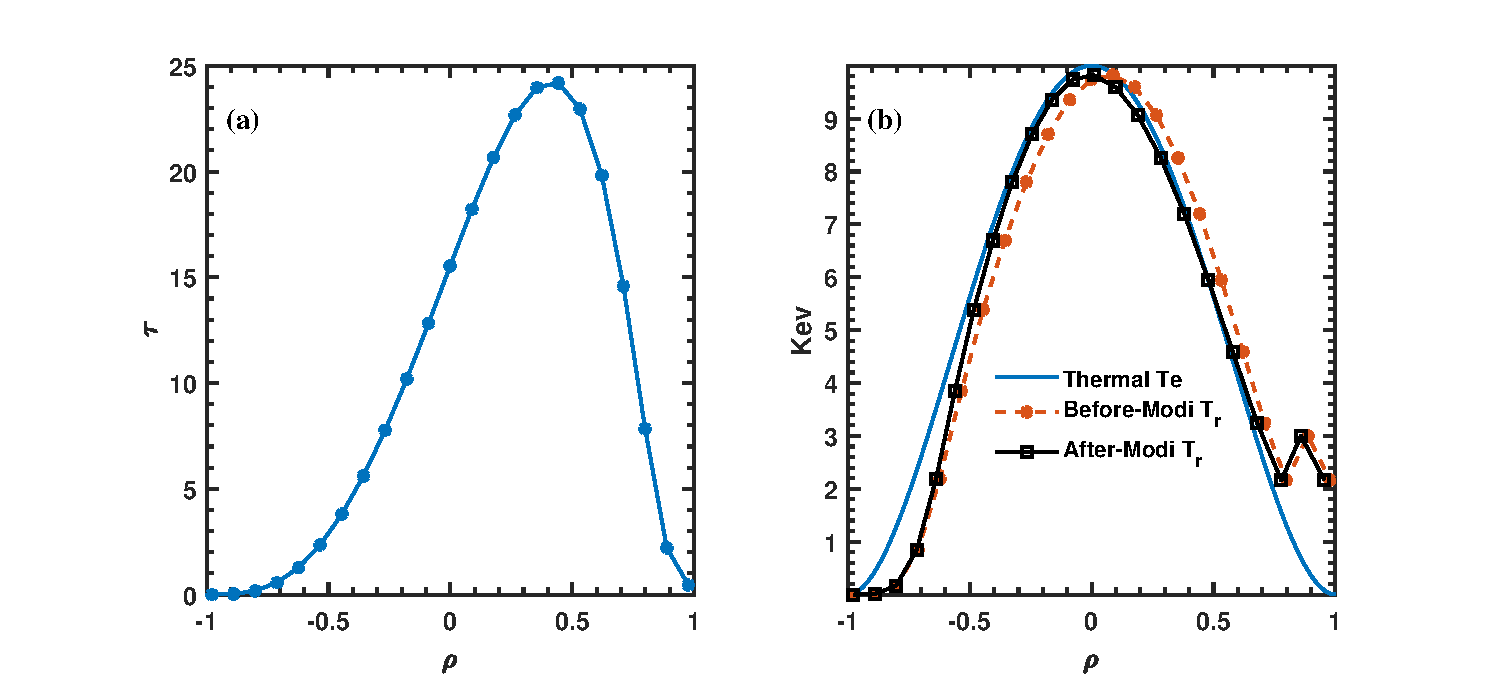
\includegraphics[width=14cm]{Tr_Modification3.eps}
\caption{\label{fig:Tr_Modification} (a)光学厚度(b)热电子温度$T_e$、修正位置前辐射温度Before-Modi $T_r$以及修正位置后的辐射温度After-Modi $T_r$}
\end{figure}
\begin{equation}
\omega=\frac{m \omega_{\mathrm{ce}}}{1-\beta_{\|} \cos \theta}=\frac{{m \omega_{\mathrm{c} 0}}/{\gamma}}{1-\beta_{\|} \cos \theta}
\end{equation}
考虑垂直磁场方向,$\theta=\pi/2$,因此
\begin{equation}
\omega=m \omega_{\mathrm{c} 0}/{\gamma}
\end{equation}
又因为$\gamma=\frac{1}{\sqrt{1-\beta^2}}$,对$\omega$关于$\beta^2$泰勒展开并取一阶近似得到
\begin{equation}
\omega=m \omega_{\mathrm{c} 0}\{1-1/2\beta^2+O(\beta^2)\}
\end{equation}
考虑电子温度为Te的等离子体中热速度$v_T=\sqrt{\frac{2T_e}{m_e}}$,取$\beta_T=v_T/c$,可得到相对论展宽为
\begin{equation}
\Delta\omega=\frac{T_e}{m_ec^2}m \omega_{\mathrm{c} 0}
\end{equation}
相对论展宽是完全下移的,非对称的,如若修正,需对每一个辐射频率所对应的位置作如下偏移:
\begin{align}
f_{rad}=f-\frac{T_r f}{m_ec^2}\\
r_{modify}=\frac{B_0R_0e}{\pi m_e f}-R_0
\end{align}
如果不考虑相对论位置修正,则对应关系为
\begin{align}
r_{raw}=\frac{B_0R_0e}{\pi m_e f_{rad}}-R_0
\end{align}
其中$f_{rad}$为辐射频率,f为实际位置冷等离子体共振频率。为了将这种修正所带来的好处展示的更加清晰,这里取芯部电子温度为10keV其它参数不变的等离子体作为计算目标,其光学厚度和辐射温度如\autoref{fig:Tr_Modification}所示,修正后的辐射温度在光学厚区域基本和实际温度吻合。此外低场侧边界位置处的小峰是辐射穿透效应,该效应将在下节展开介绍。
\subsection{超热电子存在时2X模电子回旋辐射}
现在考虑另一种情况,假设在上述等离子体背景环境中在半径$ρ_s$处存在部分超热电子成分。超热电子占当地电子数比重为$η_0$,超热电子平行方向速度为$\beta_{\parallel}$,超热电子的垂直温度和平行温度分别为$T_{s⊥0}$、$T_{s\|0}$,且超热电子温度分布与密度占比分布和当地位置满足高斯关系
\begin{align}
T_{s } & =T_{s  0} \exp \left(-\left(\frac{\rho-\rho_{s}}{d}\right)^{2}\right) \\
\eta & =\eta_{0} \exp \left(-\left(\frac{\rho-\rho_{s}}{d}\right)^{2}\right)
\end{align}
其中d表示分布展宽。为了体现超热电子对回旋辐射的影响,这里以如下超热电子参数为例:$ρ_s=-0.2$,$η_0=0.05$,$d=0.01$,$T_{s⊥0}=400KeV$,$T_{s∥0}=2KeV$,$β_∥=0.1$,如\autoref{fig:Sdistri}所示。
\begin{figure}[ht]
\centering
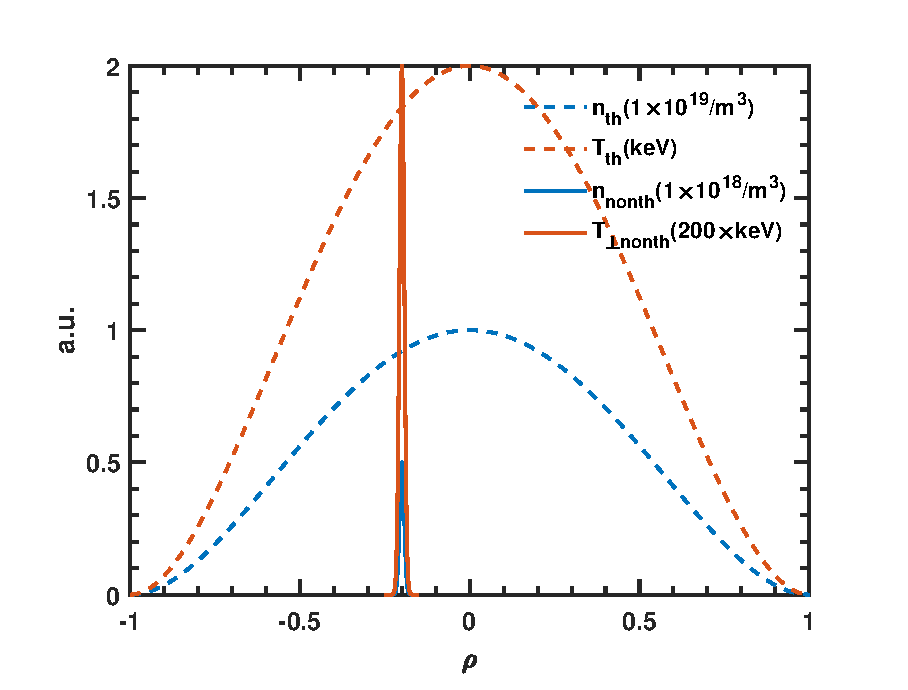
\includegraphics[width=12cm]{image60_1.eps}
\caption{\label{fig:Sdistri}等离子体中热电子及超热电子空间分布}
\end{figure}
这里分别选取143Ghz、124Ghz、 116Ghz、110Ghz、104Ghz为接收频率。
\par 如\autoref{fig:SIdistri}所示,以116Ghz紫色线为例,其对应的冷等离子体共振位置在$ρ\sim0.33$处,辐射从$ρ=-0.2$处开始增加,然后在冷等离子体共振层附近下降至接近对应位置温度的黑体辐射强度。这是因为在$ρ=-0.2$处存在超热电子,考虑超热电子温度最大为400keV,其对应的相对论展宽为$\Delta\omega=\frac{T_e}{m_ec^2}\omega_{m}$($\omega_{m}=m\omega_{c0}$,$\omega_{c0}$为静电子回旋频率),该处2X电子回旋频率$\omega_{2}=141Ghz$,相对论展宽为110Ghz,理论上该处电子回旋辐射频率在$30Ghz\sim141Ghz$区间均存在,因此会在此出现116Ghz的频率信号。除此之外124Ghz、110Ghz、104Ghz也都会从超热电子处产生。当116Ghz辐射经过冷等离子体共振层附近时,由于和背景等离子体满足共振吸收条件导致辐射信号因吸收而降低,当共振吸收足够强时,辐射会降低到黑体辐射水平(如116Ghz、124Ghz)。而当共振吸收不足以完全吸收超热电子辐射时,黑体辐射条件不再满足,接收到的辐射信号将会携带超热电子辐射成分,这时候就辐射温度就远大于电子温度。这种情况一般会在光学厚度小于1的位置出现,例如等离子体边界,如\autoref{fig:STdistri}在靠近低场侧电子辐射温度明显高于边界温度。边界辐射增强的现象一般称为辐射穿透效应,该效应早已有相关模拟和实验报道\cite{RN2065},本文通过程序重现了该过程。
\begin{figure}[ht]
\centering
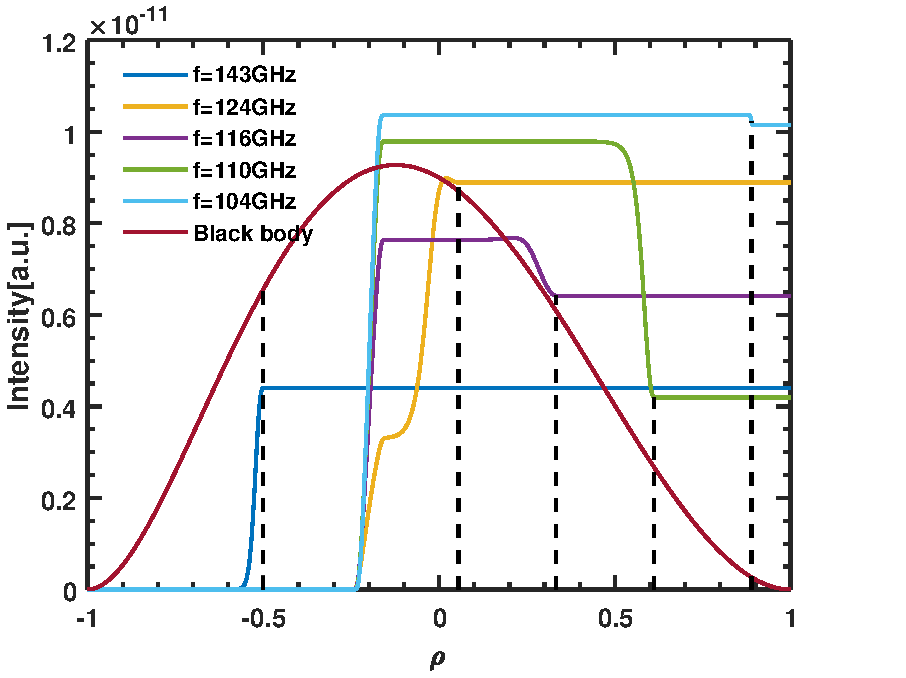
\includegraphics[width=12cm]{image61.pdf}
\caption{\label{fig:SIdistri}各频率辐射强度分布图,其中黑色虚线表示对应频率的冷等离子体电子回旋共振位置}
\end{figure}

\begin{figure}[H]
\centering
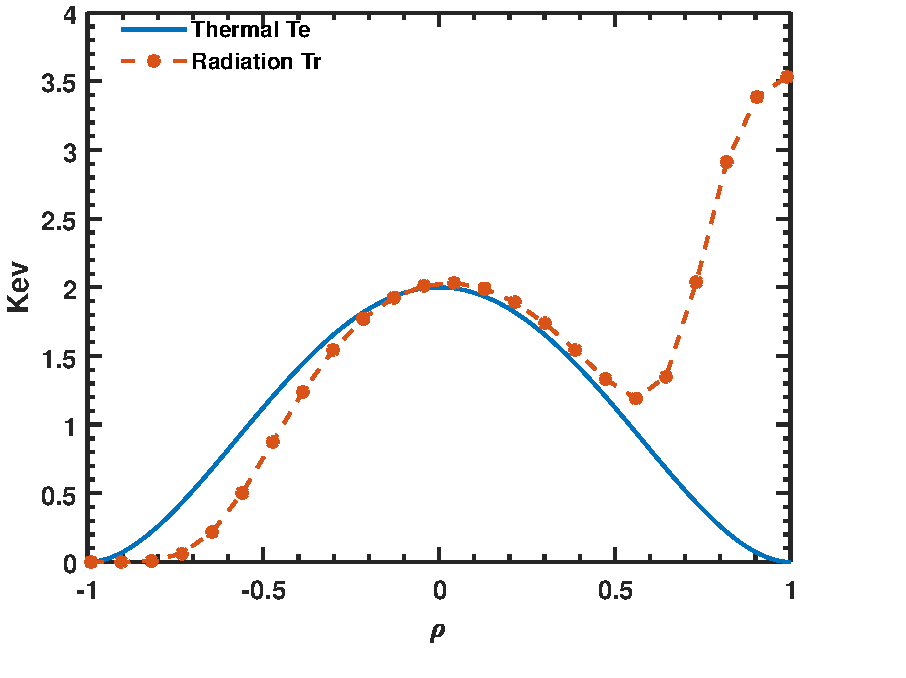
\includegraphics[width=12cm]{image62.pdf}
\caption{\label{fig:STdistri}超热电子存在下辐射温度与电子温度分布}
\end{figure}

\section{小结}
本章主要考虑稀薄等离子体环境下基于电子速度分布函数计算电子回旋辐射的问题,分别考虑了体辐射率、吸收系数以及辐射路径,结合输运方程完成了从分布函数到辐射强度正向过程的计算程序。求解过程的主要难度为二维狄拉克函数的积分,通过变基将二维狄拉克函数积分变为一维积分,实现了对辐射强度和吸收系数的求解。为了确保Trubnikov模型的准确性\cite{RN1344},本章首次对比了Trubnikov基于爱因斯坦发射吸收系数和Bornatic 基于麦克斯韦组方程得到的光学厚度\cite{RN351},验证了两种模型在处理局域热平衡等离子体时的一致性。最后本章通过开发的计算程序测试了光学厚度对辐射的影响,验证了只有满足光学厚条件时辐射强度正比与当地温度,修正了相对论效应导致辐射频率与位置对应关系的偏移,重现了当光学厚度小于1同时存在超热电子时在等离子体边界的辐射穿透效应。由于目前没有具体的非热化电子分布,只能通过双温分布定性分析非热化电子对辐射的影响,在接下来的一章里,我们主要解决非热化电子分布和演化问题。











